\documentclass[master=ecws,masteroption=ai]{kulemt}

\setup{title={Learning a Diseases Embedding using Generalized Word2Vec Approaches.  },
  author={Milan van der Meer},
  promotor={Prof.\,dr.\ R. Wuyts\and Alexander Vapirev},
  assessor={Prof. dr. ir. H. Blockeel\and R. van Lon },
  assistant={Dr. E. D'Hondt}}
% The following \setup may be removed entirely if no filing card is wanted
\setup{filingcard,
  translatedtitle=,
  udc=621.3,
  shortabstract={Here comes a very short abstract, containing no more than 500
    words. \LaTeX\ commands can be used here. Blank lines (or the command
    \texttt{\string\pa r}) are not allowed!
    \endgraf \lipsum[2]}}
% Uncomment the next line for generating the cover page
%\setup{coverpageonly}
% Uncomment the next \setup to generate only the first pages (e.g., if you
% are a Word user.
%\setup{frontpagesonly}

% Choose the main text font (e.g., Latin Modern)
\setup{font=lm}

% If you want to include other LaTeX packages, do it here. 
\usepackage{graphicx}
\usepackage{float}
\usepackage{mathtools}
\usepackage{enumitem}
\usepackage[normalem]{ulem}
\useunder{\uline}{\ul}{}
\usepackage{algorithm}
\usepackage{algpseudocode}
\usepackage{amsmath}
\usepackage{caption}
\usepackage{subcaption}
\usepackage[justification=centering]{caption}
% Finally the hyperref package is used for pdf files.
% This can be commented out for printed versions.
\usepackage[pdfusetitle,colorlinks,plainpages=false]{hyperref}
\hypersetup{%
  colorlinks = true,
  linkcolor  = black
}


%%%%%%%
% The lipsum package is used to generate random text.
% You never need this in a real master thesis text!
\IfFileExists{lipsum.sty}%
 {\usepackage{lipsum}\setlipsumdefault{11-13}}%
 {\newcommand{\lipsum}[1][11-13]{\par And some text: lipsum ##1.\par}}
%%%%%%%

%\includeonly{chap-n}
\begin{document}

\begin{preface}
 
I start with expressing my gratitude towards Roel for giving me the opportunity to work on a truly interesting subject. I also appreciate that you were not just an invisible promoter, but a promoter who showed a true interest in the subject and curiosity for the results of the research. \\
I also know that I am a lucky student who fell with his "butt in the butter" as Ellie took the time and effort to proofread my thesis a couple of times. Together with Roel, you really provided me with a lot of support and made it possible to finish my thesis in a way I'm proud of. Thank you. \\
On a  more personal note, I want to thank the people who stood by my side. My parents who gave me the opportunities in life and also prepared me for those opportunities. My friends, the CW kneusjes, my kotgenoten, and of course Siemen, the guy who somehow still manages to stay around. I also want to thank my future wife, just to cover all bases. \\

\noindent Milan out.
 
\end{preface}

\tableofcontents*

\begin{abstract}

  \lipsum[1]
\end{abstract}

% A list of figures and tables is optional
%\listoffigures
%\listoftables
% If you only have a few figures and tables you can use the following instead
\listoffiguresandtables
% The list of symbols is also optional.
% This list must be created manually, e.g., as follows:
\chapter{List of Abbreviations and Symbols}
\section*{Abbreviations}
\begin{flushleft}
  \renewcommand{\arraystretch}{1.1}
  \begin{tabularx}{\textwidth}{@{}p{12mm}X@{}}
    EHR   & Electronic Health Record \\
    ICD   & International Classification of Diseases \\
    WHO  & World Health Organization \\
    MedDRA & Medical Dictionary for Regulatory Activities \\
    THIN & The Health Improvement Network \\
    ML & Machine Learning \\
    CBOW & Continuous Bag-of-Words \\
    knn & k-Nearest Neighbors \\
    kd & k-dimensional \\
    MLP & Multilayer Perceptrons \\
    RNN & Recurrent Neural Network \\
    LSTM & Long-Short Term Memory \\
    DL4J & DeepLearning for Java \\
    MSLR & Thomson Reuters MarketScan Lab Database \\
    OMOP & Observational Medical Outcomes Partnership \\
    OSIM2 & Observational Medical Dataset Simulator Generation 2 \\
  \end{tabularx}
\end{flushleft}


% Now comes the main text
\mainmatter

\chapter{Introduction}
\label{cha:introduction}

In today's medical world, more and more data is stored using Electronic Health Records. Each time a patient goes to a hospital, doctor or receives lab results, those events are stored in the patient's Electronic Health Record. The medical world and governments are interested in EHRs as they can for example provide new insights into disease trajectories, drug treatments, medical costs, or the link between demographics and certain diseases. \\

Due to the increased usage of EHRs, a new research area emerged, namely the area of Electronic Health Record Analytics. EHR analytics is an active research field as a lot of different problems need to be solved, like different codings, privacy, interpretation, and large amounts of data. At the moment several research groups are working on utilizing EHRs to find medical patterns with several methods like querying, statistics, data mining, and artificial intelligence approaches. \\
The methods we mentioned vary from simple to very complex. In the field of machine learning algorithms, a limited amount of research is done on EHRs, mainly using out-of-the box tools. \\
The focus point of this thesis is: applying advanced machine learning algorithms to find patterns in EHRs. \\

An EHR of a patient can be seen as a time series, namely a sequence of EHR events such as visits to the doctor. In this thesis we make the analogy between sentences of words and sequences of EHR events. Based on this analogy, we propose novel techniques which are generalizations of the Word2Vec approach, a technique typically used in linguistic analysis \cite{w2vOriginal:article}. \\
To enable this, we use several prepocessing methods. One of these methods is a newly proposed disease code mapping between two standards namely MedDRA and ICD-10. This mapping is used to categorize diagnoses and to make our validation process possible.\\ 
We also categorize our EHR events into more general events. For example, a bruise on your right leg and a bruise on your left leg should both be categorized under a bruises event. \\

We introduce generalized Word2Vec. This generalized Word2Vec makes it possible to apply Word2Vec on medical data. \\
To make these approaches possible for large-scale medical datasets, we apply the generalization concept on DeepWalk. DeepWalk makes it possible to generate a smaller dataset from the original dataset and then apply a Word2Vec approach on this smaller dataset for performance reasons. \\
Besides the exploration on generalizing Word2Vec approaches, we also improve Word2Vec by tackling one of its shortcomings. This shortcoming of Word2Vec is that it is unable to handle unseen instances once it has built his model. We combine a k-nearest neighbors method with Word2Vec and make an estimation of the correlation to other diagnoses for the unseen instance. \\

We compare the model from our Word2Vec methods applied on a OSIM2 dataset to the results of the currently largest study on Danish EHRs \cite{Brunak:article}. The OSIM2 dataset is a simulated dataset generated by an organization named OMOP. \\
To make it possible to apply our methods on the OSIM2 dataset, we use the above mentioned disease code mapping. \\

Within the limitations of our validation method, we conclude that our model does match the Danish results well depending on how the matching is defined. Especially since we use several estimations such as the disease code mapping, different datasets, and categorization. \\

The structure of this thesis is as follows. In chapter \ref{cha:context}, we describe the general field of EHR and EHR analytics. We also introduce the relevant state of the art. In chapter \ref{cha:background}, we provide the background needed to understand our generalized Word2Vec approaches and afterwards describe our novel techniques. In chapter \ref{cha:implementation}, we describe how we make a model of the OSIM2 dataset using our proposed techniques and how to validate our model. In chapter \ref{cha:futureWork}, we mention some possible improvements and extensions left to explore.

%%% Local Variables: 
%%% mode: latex
%%% TeX-master: "thesis"
%%% End: 

\graphicspath{ {Context/Images/} }


\chapter{Context}
\label{cha:context}

\section{Introduction}
In this chapter 

Context: Depends on chosen problem (Extracting knowledge from EHR )

	Problem: info out of EHR
	State of the art:
	
		Explain Disease codes
		DiseaseProgression
		Explain Danish paper, Matrix group America (recommender), Querying


\section{Electronic Health Records}

An electronic health records (EHR) is a collection of data about a patient at a certain point in time. It is stored digitally and thus can be part of a large number of patients over a long time period.

\subsection{Disease Codes}

An important part of EHRs is applying methods which are uniform and well documented. This makes it easy to store and extract data from large-scale databases of EHRs. A part of an EHR consists of the diagnosis of the patient. It provides information about the disease trajectory of the patient and allows analysis on the health situation of a patient. With a uniform system for classifying diseases, it is possible to provide a general picture on health situations of populations.

\subsubsection{ICD-10}

The International Statistical Classification if Diseases and Related Health Problems (ICD) is a medical classification list made by the World Health Organization (WHO). The ICD contains more than $14,400$ codes about diseases, disorders, injuries, and other related health conditions. It also provides hierarchical categories for those codes to allow a more general overview of diseases.


\subsubsection{MedDRA}

The Medical Dictionary for Regulatory Activities (MedDRA) provides medical terminology in the form of disease codes. It doesn't provide hierarchical categories.

\section{EHR Analytics}

EHRs provide a massive amount of data which could be used to create useful insights. Those insights can be offered on an individual level, which means a right intervention to the right patient at the right time. EHR analytics can be used to have a personalized care for patients and benefits the healthcare system by cutting costs and improved outcomes. \\

In the following sections we talk about current EHR analytic methods.


\subsection{Querying}



\subsection{Recommender Systems}

\subsection{Statistical Analysis}

\subsection{Patient Similarity}


http://www.who.int/classifications/icd/en/

http://arxiv.org/pdf/1112.1668v1.pdf

https://en.wikipedia.org/wiki/Electronic\_health\_record#Technical\_features

file:///media/milan/Data/Chrome\%20Downloads/EHRAnalytics_Stateoftheart\%20(1).pdf

http://www.meddra.org/

https://www.siam.org/meetings/sdm13/sun.pdf

Jimeng Sun, Fei Wang, Jianying Hu, Shahram Edabollahi: Supervised patient similarity measure of
heterogeneous patient records. SIGKDD Explorations 14(1): 16-24 (2012)


\section{Conclusion}
The final section of the chapter gives an overview of the important results
of this chapter. This implies that the introductory chapter and the
concluding chapter don't need a conclusion.



%%% Local Variables: 
%%% mode: latex
%%% TeX-master: "thesis"
%%% End: 

\graphicspath{ {Background/Images/} }


\chapter{Generalized Word2Vec}
\label{cha:background}

\section{Introduction}
In this chapter we introduce important concepts which are needed to understand our approach. These concepts can be used to solve problems described in chapter \ref{cha:context}. \\

We start with explaining some background knowledge in section \ref{sec:bk} such as time series and machine learning. We focus on basic concepts from machine learning and then focus more on neural networks. The main part to understand our approach is the introduction of Word2vec in section \ref{sec:word2vec}. This is then used to introduce Deepwalk as an extension on Word2Vec in section \ref{sec:deepwalk}. \\

After introducing those concepts, we explain our generalized word2vec approaches in section \ref{sec:gw2v}.


\section{Background Knowledge}
\label{sec:bk}

	\subsection{Time Series Analysis}
A time series consists of data points over a certain time period. We refer to this as a sequence of states. Where a state represents a data point and can differ from a single value to more complex representations like pictures. \\
The domain of time series analysis handles around extracting information or relations from a time series. It can have different goals like forecasting, classification, or exploratory. \\

A medical history of a patient can be seen as a time series, namely a sequence of EHRs. This means that methods which are applied on time series, are also applicable on medical data to find patterns.

	\subsection{Machine Learning}
Machine learning is a data driven approach with as goal to build a model which can be	used to make predictions or decisions. Note that this model can be used to predict outcomes of time series. This task is done by algorithms which are able to learn models based on examples given by the designer. Based on the examples, machine learning aims to tackle $3$ types of problems, namely supervised learning, unsupervised learning, and reinforcement learning. \\
Supervised learning is concerned with the learning task where there are examples given with their corresponding label. Unsupervised learning is similar to supervised learning only no labels are given. We won't go into reinforcement learning. \\
We can also classify the problems according to the desired output of our model. Those main tasks consist of classification, regression, and clustering. \\
	
We mention some used methods in the field of machine learning. These are used in above mentioned problems. \\
In the field of classification neural networks are used to achieve state of the art results. For regression, support vector machines can be used. One of the most popular methods for clustering is K-means. 

	\subsection{K-nearest Neighbors}
	\label{sec:knn}
	
The k-Nearest Neighbors (knn) algorithm is a simple machine learning algorithm \cite{knn:article}. It will be used in our generalized Word2Vec approach. \\
When you are in a supervised context, you have several instances with labels. When you retrieve a new instance, you want to predict its label. Based on a defined similarity measure (ex. Euclidean distance), you can look for the $k$ nearest labeled instances distanced to the new instance. From those, you pick the most common label in the pool of the $k$ nearest instances. This label becomes your predicted label for the new instance.
	
	
	\subsection{K-dimensional Tree}
	\label{sec:kdtree}
	
A naive way to calculate the nearest neighbors for a new element in a vector space, is by comparing all members with the new element and keep track of those distances. \\
A more efficient way is to use a k-dimensional tree (kd tree) \cite{kdtree:article}. In this section we explain the workings of this approach in more detail \cite{kdtreeIntro:atricle}. \\

A kd tree is a way of storing k-dimensional points. It is a binary tree where each node represents an element in the vector space. The node also contains information on how the tree is split up. It keeps track of the plane it is split on and the left and right sub tree. In figure \ref{fig:kdtreeSplit} you can see an example on how a simple kd tree is made and how it splits up the x,y plane. In the upper figure, the splitting plane is not mentioned, it is the $y=5$ plane for the $[2,5]$ and $x=3$ for $[3,8]$. \\
	
\begin{figure}[!htb]
	\centering
	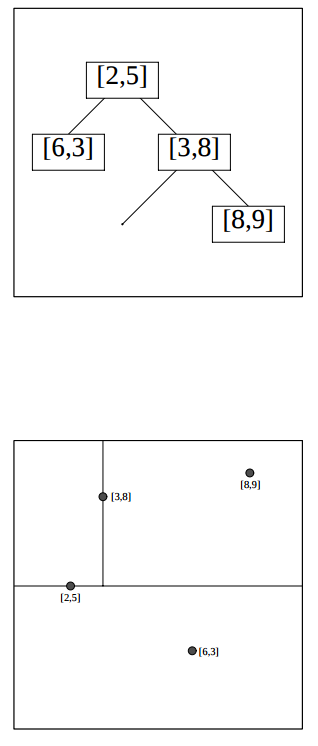
\includegraphics[width=0.4\textwidth]{kdtreeSplit.png}
	\caption{Representation on how a binary kd tree splits up the plane  \cite{kdtreeIntro:atricle}}
	\label{fig:kdtreeSplit}
\end{figure}

Now that we can construct the kd tree, we can use it to find the nearest neighbor for a certain input point. \\
We start with root node and recursively go down the kd tree. At each node it goes to the left or right depending on if the input is lesser or greater than the current nodes value on the splitting plane. Once it reaches a leaf node, it marks this node as the current nearest neighbor. \\
The algorithm unwinds the recursion of the tree, performing the following steps at each node:
\begin{itemize}

\item If the current node is closer than the current best, then it becomes the current best.
\item It checks if it is possible whether there is the possibility of closer points on the other side of the splitting plane. It makes a hypersphere around the current node with a radius equal to the current nearest distance. 
\begin{itemize}
\item If the hypersphere crosses the splitting plane, there could be a closer point on the other side. This means the algorithm will move down the other branch of the current node.
\item If the hypersphere does not cross the splitting plane, the whole other branch can be skipped.
\end{itemize}
\end{itemize}

This algorithm is easily extended to find the k-nearest neighbors by keeping track of the k current bests.
	
	\subsection{Neural Networks}
	
A neural network is a machine learning approach based on biological neural networks. It can be used to find patterns and do predictions on time series. Those time series can be medical data.


		\subsubsection{Perceptron}

The basic component of a neural network is a perceptron \cite{perceptron:article}. A perceptron takes multiple binary inputs and has a single binary output (see figure \ref{fig:perceptron}). Each input has a corresponding real numbered weight $w_j$. The output is decided on the following equation: \\

\begin{equation} 
output =
  \begin{cases}
    0       	& \quad \text{if } \sum_j w_jx_j \leq \text{ threshold}\\
    1  		& \quad \text{if } \text{if } \sum_j w_jx_j > \text{ threshold}\\
  \end{cases}
\end{equation}
	
\begin{figure}[!htb]
	\centering
	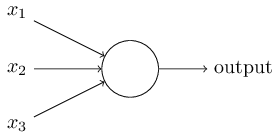
\includegraphics[width=0.4\textwidth]{perceptron.png}
	\caption{Simple presentation of a perceptron \cite{NNintro:online}}
	\label{fig:perceptron}
\end{figure}

We can build a network by connecting multiple perceptrons (see figure \ref{fig:multiplePerceptrons}). By building these networks, more complex decisions can be made. The reason for this, is that once there are atleast $3$ layers of perceptrons (and non-linear activation functions), the network can find non-linear relations between the input and output \cite{nnNL:article}. \\

\begin{figure}[!htb]
	\centering
	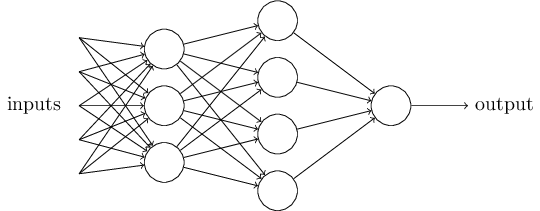
\includegraphics[width=0.8\textwidth]{multiplePerceptrons.png}
	\caption{More complex network made by connecting multiple perceptrons \cite{NNintro:online}}
	\label{fig:multiplePerceptrons}
\end{figure}

Now we have seen how a general network is constructed, we look at some vocabulary. \\
In figure \ref{fig:networkArch}, we see a four-layer network. As mentioned on the figure, we call the first layer the input layer, the last layer the output layer, and the layers in between are called hidden layers. Sometimes a multiple layer network is referred to as multilayer perceptrons or MLP. 

\begin{figure}[!htb]
	\centering
	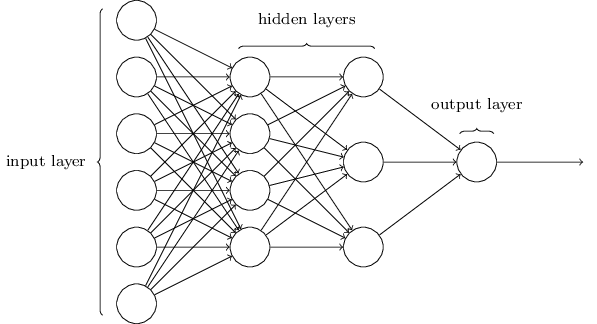
\includegraphics[width=0.8\textwidth]{networkArchitecture.png}
	\caption{General vocabulary of a multilayer network \cite{NNintro:online}}
	\label{fig:networkArch}
\end{figure} 		


		\subsubsection{Training a network}
		
To train a neural network, we input an example with a known label. The network will calculate a certain output based on the current weights. When this output is incorrect, it should be possible to adjust the weights with as effect that the network now has as output the correct label. Note that the change in weights, should only effect the output by a small bit (see figure \ref{fig:smallChange}). The reason for this is that otherwise all the previous inputs could now be labeled incorrectly. So, the concept of training a neural network means, adjusting the weights in a way that the behavior of the network doesn't change completely on the previous seen examples but that the current examples is labeled correctly. \\

\begin{figure}[!htb]
	\centering
	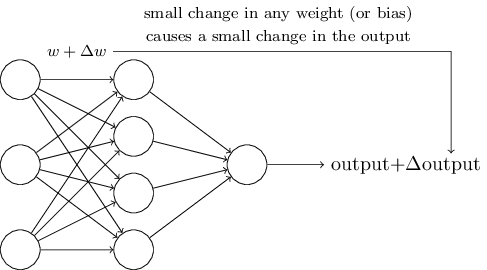
\includegraphics[width=0.8\textwidth]{smallChange.png}
	\caption{Small change on the weights, only has a small impact on the output \cite{NNintro:online}}
	\label{fig:smallChange}
\end{figure} 

To achieve this effect, we change our above explained perceptrons to sigmoid neurons. A sigmoid neuron has the same basics as a perceptron. It still has inputs but now it also has a bias $b$. The inputs still have weights but the weights can now range between $0$ and $1$. The output is now calculate with $\sigma(w*x+b)$ where $\sigma$ is the sigmoid function. This results in the following formula: 

\begin{equation} 
\frac{1}{1+exp(-\sum_j w_jx_j-b)}
\end{equation}

\noindent The sigmoid function makes it possible to calculate the gradient and makes the output a linear combination of $\Delta w_j$ and $\Delta b$ as $\Delta output$ is approximated by 

\begin{equation} 
\Delta output \approx \sum_j \frac{\partial output}{\partial w_j}\Delta w_j + \frac{\partial output}{\partial b}\Delta b
\end{equation}

\noindent Because of the linearity, it is now easier to choose changes for the weights and biases to achieve a correct output. By adjusting the weights, we will train our network to achieve a higher accuracy on the seen examples.
		
	\subsection{Backpropagation}
	
Backpropagation is an algorithm which is used to train neural networks \cite{bp:article}. It calculates the gradient of a chosen cost function with respect to the individual weights. Based on the gradient, the weights are updated and the cost function is minimized.

		\subsubsection{Terminology}
		
We use $w^l_{jk}$ to denote the weight corresponding to the connection between the $k^{th}$ node in the $(l-1)^{th}$ layer and the $j^{th}$ node in the $l^{th}$ layer. We use $b^l_j$ for the bias of the $j^{th}$ node in the $l^{th}$ layer and $a^l_j$ for the activation of the $j^{th}$ node in the $l^{th}$ layer. See figure \ref{fig:termNN}. \\

\begin{figure}[!htb]
	\centering
	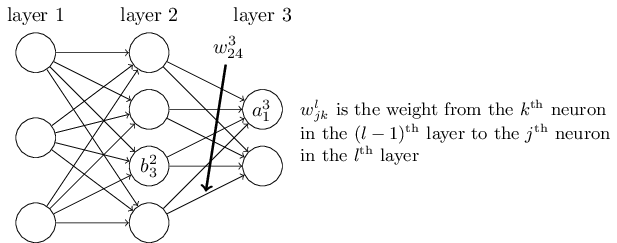
\includegraphics[width=0.8\textwidth]{termNN.png}
	\caption{Visual representation of the terminology for a neural network \cite{NNintro:online}}
	\label{fig:termNN}
\end{figure} 

\noindent We can now convert this notation to a vector representation. We remove the indexes for the node numbers which results in the following:

\begin{equation} 
a^l = \sigma (w^la^{l-1}+b^l)
\end{equation}

		\subsubsection{Cost function}
		
As mentioned before, backpropagation has as goal to calculate the partial derivatives of the cost function $C$ with respect to each weight and bias. \\
The cost function has to fulfill certain criteria. The first one is that it needs to be possible to write it as a summation over cost functions for individual training examples. Secondly, it needs to be derivable. And lastly, the cost function is a function of the activations of the last layer. 


		\subsubsection{Fundamental equations}

Backpropagation has 4 equations. They allow us to calculate the error for each node and adjust the weights based on the gradient descent. \\

First we calculate the error of each node which is based on how much the cost function is influenced by each activation and on how much the activation function is influenced by $z_j^L$:

\begin{equation} 
\delta^L_j = \frac{\partial C}{\partial a^L_j} \sigma'(z_j^L)
\text{ with }
z_j^L = \sum_k w^L_{jk}a^{L-1}_k+b^L_j
\end{equation}

\noindent This can be written as a neat vector equation:

\begin{equation} 
\delta^L = (a^L-y) \circ \sigma'(z_j^L)
\end{equation}

\noindent The next equation explains why the algorithm is called backpropagation. The equation calculates each layers error vector based on the layer after it, it propagates the error back over the layers:

\begin{equation} 
\delta^l = ((w^{l+1})^T\delta^{l+1}) \circ \sigma'(z_j^L)
\end{equation}

\noindent With those 2 equations we calculate the error in each layer of the neural network. Those errors can be used to calculate the derivatives of the cost function with respect to the weights and the biases:

\begin{equation} 
\frac{\partial C}{\partial w^l_{jk}} = a^{l-1}_k \delta^l_j.
\end{equation}

\begin{equation} 
\frac{\partial C}{\partial b^l_j} = \delta^l_j.
\end{equation}

\noindent When the derivatives are calculated, we can apply the gradient descent and update the weights and biases accordingly. This process represents the learning of a neural network.


\section{Word2Vec}
\label{sec:word2vec}

\subsection{Motivation}

We will explain Word2Vec in this section. It is explained from a linguistic point of view. This explanation is needed to introduce our generalized Word2Vec approach which can be applied to medical data. \\

In natural language processing tasks, a good representation of words helps learning algorithms perform better. A representation is learned which maps words to vectors in a low-dimensional space compared to the vocabulary size. In this representation, we try to map context-similar words close to each other in the new vector space. The new representation is sometimes also called a 'word embedding'. \\
We could say in an informal way: a linguistic background is made which the learning algorithm can use. \\


\subsection{Skip-gram}

There are two main models used for word2vec \cite{w2vOriginal:article}, namely Continuous Bag-of-Words (CBOW) and the Skip-Gram model. \\
The first one tries to predict a word if a context is given (ex. predict Paris when capital France is given). And the second one does the inverse of this approach \cite{w2vModels:article}. Empirical results have shown that the Skip-Gram model tends to do better on larger datasets \cite{w2vReason1:online} and gives a better representation for infrequent words \cite{w2vArchive:online}. In medical data there are often infrequent cases which are important. For those reasons, we choose to go further with the Skip-Gram model. \\

So one way of learning a word2vec representation of a corpus $Text$, is by using the skip-gram model. \\
Based on given words $w$ and their contexts $c$, we set the parameter $\theta$ of $p(c|w;\theta)$ to maximize:

\begin{equation} 
\arg \max_{\theta} \prod_{(w,c \in D} p(c|w;\theta)
\end{equation}

\noindent with $D$ the set of all word and context pairs we extract from the corpus.\\
Here we also note that $p(c|w)$ is indeed the chance of a context appearing after seeing a specific word as mentioned before.

\subsubsection{Finding word-context pairs}

Given a sequence of words, we define their context based on n-gram \cite{w2vNgram:article}. In figure \ref{fig:ngram}, n-gram is explained on the sentence "This is a sentence". 

\begin{figure}[htbp]
	\centering
	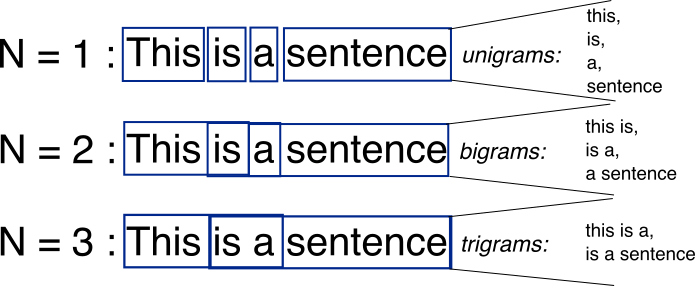
\includegraphics[width=0.8\textwidth]{ngram.png}
	\caption{Explanation of n-gram \cite{w2vNgram:online}}
	\label{fig:ngram}
\end{figure} 

For the Skip-gram model, we define the context of a word $w_t$ as $w_{t+j}$ with $j$ between $-c$ and $c$. A larger $c$ results in more training examples and thus can lead to a higher accuracy but will have a longer training time.


\subsubsection{Parameterization}

We start with rewriting the conditional probability using soft-max:

\begin{equation} 
p(c|w;\theta) = \frac{e^{v_x*v_w}}{\sum_{c' \in C}e^{v_{c'}*v_w}}
\end{equation}

\noindent where $v_c$ and $v_w$ are vector representations for $c$ and $w$, and $C$ is the set of all available contexts. This means that the parameters $\theta$ are $v_{c_i}$ and $v_{w_i}$. Computing the optimal parameters is very expensive because you need to calculate this over all contexts $c'$. We also switch from product to sum by taking the logs:

\begin{equation} 
\arg \max_{\theta} \sum_{(w,c) \in D} \log p(c|w;\theta) = \sum_{(w,c) \in D} (\log e^{v_c * v_w} - \log \sum_{c'} e^{v_{c'}*v_w})
\end{equation}

\subsection{Negative Sampling}

To compute the vectors using the Skip-gram model more efficiently, we introduce negative sampling \cite{w2vExplained:article}. \\
Instead of calculating $\sum_{c' \in C}e^{v_{c'}*v_w}$ over all contexts, we make a set $D'$ which consists of randomly sampled word-context pairs. With this new set, we remove the costly term $\sum_{c' \in C}e^{v_{c'}*v_w}$ and replace it with $\sum_{(w,c) \in D'}e^{v_{c'}*v_w}$. \\

In a less formal way: we are not making sure that if words appear in the same context, their vectors are more similar than all the other word vectors, but only of several vectors chosen randomly. This makes the Skip-gram model usable in terms of speed.


\subsection{Neural Networks}

When the word2vec algorithm is trained using the Skip-gram model, one will have a lookup table. This table contains the mapping of words to their vector representation. This lookup table can be found by training a 2-layer neural network with as goal function the function described in the previous section. The training can be done with Gradient Descent for example. \\
The trained 2-layer neural network can be placed in front of another neural network \cite{w2vNN:online}. It will convert the words to their vector representation and feed into the next neural network. It is empirically shown that this can improve the results of the neural network by putting the lookup table in front of it. As mentioned before, in a way, you offer background knowledge to the neural network.

\section{DeepWalk}
\label{sec:deepwalk}

DeepWalk is an approach where graph structured data is transformed into sequences of vertices \cite{deepwalkMain:article}. Word2vec is then applied on those sequences to learn a good vector representation for the vertices. We can say that it is an extension on the Word2Vec approach. \\

In figure \ref{fig:dwAlgo}, we see an overview of the DeepWalk algorithm. It exist of two parts. 

\begin{figure}[!htb]
	\centering
	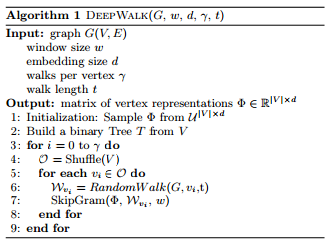
\includegraphics[width=0.7\textwidth]{dwAlgo.png}
	\caption{Overview of the DeepWalk algorithm \cite{deepwalkMain:article}}
	\label{fig:dwAlgo}
\end{figure} 

First a random walk generator. For each vertex $v_i$ of the graph $G$, it will generate a random walk of length $t$. It will do this $\gamma$ times but the order to which the vertices are traversed, is randomly ordered each pass. With those walks, a sequence of vertices is generated. \\
Secondly, those vertices are used for word2vec. This process is explained in section \ref{sec:word2vec}.


\section{Generalized Word2Vec Approaches}
\label{sec:gw2v}

In this section we explain our approach on how to find patterns in EHRs. For this, we use generalized Word2Vec approaches to learn disease embeddings. 

\subsection{Data representation}

Before we can start with explaining how Word2Vec can be applied on EHR data, we start with introducing our data representation. \\
The medical history of a patient is a time series of EHRs. On certain timestamps, an EHR is available containing the medical state of that patient. We call this EHR the vector $m^p_t$, with $p$ a patient number and $t$ a timestamp. This means that each patient has a sequence of vectors $s^p = m^p_t, m^p_{t+1}, m^p_{t+3}, \ldots$. Each vector contains certain values depending on the EHRs. It can contain values for the timestamp, demographics, blood pressure, diagnoses, and others. 

\subsection{Generalized Word2Vec}

As explained in section \ref{sec:word2vec}, Word2Vec is applied on a large text corpus containing a large amount of sentences. After applying this method, an embedding is found that represents words in a new vector space. In this vector space the relationship between words is shown by the distance of the words from each other. \\

A large medical dataset containing EHRs for different patients, can be seen as a large text corpus. It contains patients, each having a sequence $s^p$, which is equivalent to one sentence. All the different patients sequences, make the whole dataset similar to how sentences make a text corpus. Each vector $m^p_t$ is removed from its link to the patient and his timestamp to make it not unique anymore, we call this vector $m$. This is to make the link to words. Different sentences can contain the same words, similar to how the vectors $m$ are in the different sequences. \\

With those links, it is possible to apply Word2Vec not only to simple objects like words, but also on more abstract objects like vectors. We call this a generalized Word2Vec approach. From this, we can learn an embedding for the vectors $m$ in the new vector space. In this new vector space, the relationships between the vectors $m$ are found based on their occurrences with others in the sequences.


\subsection{K-Nearest Neighbors Word2Vec}

A problem with using an embedding which is found on a certain dataset, is that it is possible that certain instances are not present in the dataset. In the case of a complete new instance, a Word2Vec model cannot find a representation for this instance. As we are working in the context of a generalized Word2Vec approach, where instances are represented by complex objects like vectors, the chances of this happening increases. It increases because there are a lot more possible combination of vectors possible than there are words in a dictionary for example. \\

Therefore we introduce a K-Nearest Word2Vec approach. As we are working with more abstract objects, namely vectors, we can extend our generalized Word2Vec approach with a knn feature (see section \ref{sec:knn}). After the training of a Word2Vec model, we have learned a lookup table which maps a known vector $v_{old}$ to his new vector representation $v_{new}$. When a not-yet-seen vector $v_{unknown}$ needs to be mapped to his $v_{new}$, a normal Word2Vec is not capable of this. \\
With our approach, the knn are found using a kd tree (see section \ref{sec:kdtree}). Those knn are found from all the known vectors in their old representation $v_{old}$ in the lookup table. From the new vector representations $v_{new}$ of the knn, a weighted average is taken to find the $v_{new}$ for $v_{unknown}$. \\

In short: we look for the knn of the $v_{unknown}$ from all the known vectors in their original representation $v_{old}$. Based on the found knn, we take an weighted average of the new representation $v_{new}$ from those found knn. This weighted average is the $v_{new}$ for the $v_{unknown}$.

\subsection{Generalized Deepwalk}

Deepwalk itself is hard to apply on EHR data as it starts from a graph structure. It however provides an extra Word2Vec approach which can be generalized to more abstract objects like vectors. \\

One application of Deepwalk is the need for less data to achieve a good Word2Vec model. When the EHR data becomes very large, it would take a considerable amount of time to train a Word2Vec model. Therefore it would be interesting to transform the EHR data into a weighted graph structure. The weights are based on the frequency of diagnoses following each other. \\
After the graph transformation, the amount of weighted random walks can be limited to create a smaller set of sequences based on the original dataset. Those sequences can be used to train a Word2Vec model faster as there is fewer data. The same logic from the previous two sections is applicable to generalize deepwalk from words to more abstract objects.


\section{Conclusion}
In this chapter we talked about general machine learning concepts and focused on Word2Vec. We conclude that Word2Vec is used to find good representation of words based on their context. It also causes that similar words will be close to each other in this new representation. \\

With the concepts explained, we introduced our approaches. We extended Word2Vec so that it can handle more abstract object than words, namely vectors representing an EHR. We also extended Word2Vec to find a representation for a new instance based on knn. The same extension can be done for Deepwalk.



%%% Local Variables: 
%%% mode: latex
%%% TeX-master: "thesis"
%%% End: 

\graphicspath{ {Implementation/Images/} }


\chapter{Implementation}
\label{cha:implementation}

\section{Introduction}
In this chapter 

OSIM
TensorFlow
DL4J


\section{OSIM}

In our word2vec approach we applied generalization on the medical states. This was needed to retrieve more general n-grams. For this generalization, we divided some attributes into specific intervals.

Instead of dividing some attributes into specific intervals, we could apply normalization to it. Based on the distribution of the data, we can make more sensible intervals and assign them to the attributes.


\section{TensorFlow}

Word2vec can be made distributed as the underlying idea is quite simplistic, it counts occurrences of n-grams. Counting occurrences based on labels, is a well known problem and is often solved by MapReduce algorithms. 


\section{DeepLearning4Java}

As mentioned in section \ref{sec:word2vec}, a trained 2-layer neural network can be placed before another neural network and function as a lookup table. In this section, we discuss a possible neural network which allows us to further investigate the effectiveness of our word2vec approach to classify patients. More concrete: we should check if a better accuracy is acquired with the lookup table in front of the neural network or without. 



\section{Conclusion}
The final section of the chapter gives an overview of the important results
of this chapter. This implies that the introductory chapter and the
concluding chapter don't need a conclusion.



%%% Local Variables: 
%%% mode: latex
%%% TeX-master: "thesis"
%%% End: 

\chapter{Conclusion}
\label{cha:conclusion}

This thesis started with explaining the new research area of Electronic Health Record Analytics. We explored the possible impact of this area as it allows to find medical patterns on a large scale. Those patterns range from drug discovery, disease progression for individuals, and reducing medical costs. At the moment several research groups are working on utilizing EHRs to find medical patterns using several methods like querying, statistics, data mining, and artificial intelligence approaches. \\
Our research sought to explore the usage of new machine learning approaches to find correlations between different diagnoses. The correlations found can be used in combination with prediction or classification methods. \\

We introduced a new way on how to apply Word2Vec methods by explaining the link between sentences of words and sequence of medical records. We call this approach a generalized Word2Vec approach and it can be applied on medical data to the correlations between different diagnoses. \\
To make sure the generalized Word2Vec methods can be applied to large-scale medical data, we applied the generalization concept also on DeepWalk. DeepWalk makes it possible to generate a smaller dataset from the original dataset and then apply a Word2Vec approach on this smaller dataset. \\
Besides the exploration on generalizing Word2Vec approaches, we also improved Word2Vec by tackling on of its shortcomings. This shortcoming of Word2Vec is that it is unable to handle unseen instances once it has built his lookup table. We combine a k-nearest neighbors method with Word2Vec and make an estimation of the correlation to other diagnoses for the unseen instance. \\

EXPERIMENTS + Limitations of the experiment

CONCLUSION

For more information about another possible experiment which also combines the Word2Vec approaches with prediction or classification methods, we refer to the next chapter. In this chapter we also talk about some possible improvements and future directions to explore.

%%% Local Variables: 
%%% mode: latex
%%% TeX-master: "thesis"
%%% End: 

\graphicspath{ {FutureWork/Images/} }


\chapter{Future Work}
\label{cha:futureWork}

In this thesis we explained our generalized Word2Vec approaches which we use to find disease relations in EHRs. We tested the influence of the chosen parameters on the matching percentage between the clusters found in the Danish paper and our own clusters. In the previous chapters, we already mentioned some possible roads to explore like a better disease code mapping strategy or extensive parameter tuning. \\

In this chapter we discuss possible improvements and further research which can be added to the current approaches. As mentioned in section \ref{sec:word2vec}, we can use our Word2Vec method to improve the accuracy of a predictive/classification neural network. In this chapter, we mainly discuss the predictive/classification neural network which allows us to further investigate the effectiveness of our Word2Vec approach. \\
The usage of a predictive/classification neural network in combination with our Word2Vec approaches, would make it possible to more thoroughly investigate the effects of our methods. \\

The structure of this chapter is as follows. In section \ref{sec:categorization} we discuss an improvement on how we handled categorization of medical data which we discuss in section \ref{sec:categorizationImpl}. In section \ref{sec:distributed}, we introduce an optimization for our Word2Vec approaches by utilizing data distribution. In section \ref{sec:PatientClassification}, we explain a specific neural network which can use the found patterns by the Word2Vec approaches to predict or classify patients' disease trajectories.


\section{Categorization}
\label{sec:categorization}

In our Word2Vec approaches, we applied categorization on the medical states to reduce the amount of infrequent states. This was needed to retrieve more general n-grams. For this categorization, we divided attributes like age into predefined intervals without any knowledge about the data distribution. \\

Instead of dividing attributes into predefined intervals, we could apply normalization to those attributes. Based on the distribution of the data, we can make more sensible categories and assign them to the attributes accordingly. This could lead to better divided categories and make sure outliers get a specific category.


\section{Distributed Word2Vec}
\label{sec:distributed}

Word2Vec can be made distributed as the underlying idea is quite simplistic, it counts occurrences of words in the text corpus. Counting occurrences based on labels, is a well known problem and is often solved by MapReduce algorithms \cite{mapreduce:article}.


\section{Patient Classification}
\label{sec:PatientClassification}

As mentioned in section \ref{sec:word2vec}, a trained 2-layer neural network can be placed before another neural network and the former functions as a lookup table. In this section, we discuss the latter neural network which allows us to further investigate the effectiveness of our Word2Vec approach to better classify or predict patients. More concrete: we could check if a better accuracy is acquired with the lookup table in front of the prediction/classification neural network or without the lookup table. 

\subsection{Problem Definition}
\label{sec:problem}

The medical history of a patient is a time series with as datapoints EHR events. We want to classify these time series into different types of disease trajectories. A patient who is classified into a specific disease trajectory, can be treated more specifically as we would have a better view what the next stages of the trajectory could be. In this way, classification also serves as a predictive model. \\

The medical data of multiple patients is a $3$ dimensional tensor (multi-dimensional matrix), see figure \ref{fig:rnnData}. In the figure, the examples are all the different sequences from the EHRs. The sequence length are the number of events in that sequence. And each event is a time step represented by a vector. \\
This data structure is the input structure for a neural network. \\

\begin{figure}[!htb]
	\centering
	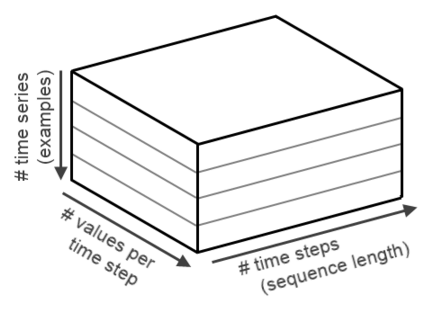
\includegraphics[width=0.8\textwidth]{rnnData.png}
	\caption{Overview of the data structure for medical data with a time aspect \cite{dl4jRnn:online}}
	\label{fig:rnnData}
\end{figure} 

Medical data has some problems which we will discuss.\\
It often consists of long time periods. This means there could be a long range of dependencies between events. In the context of training neural networks, this can cause a problem known as the vanishing gradient problem \cite{vanishingproblem:article}. \\
Patients do not have regular intervals in their medical data. The irregular intervals need to be transformed into regular intervals otherwise the time aspect will not be consistent throughout the data. \\
Standardization of attributes needs to be taken into account. For example each EHR has to use the same method to represent the diagnoses. Preferably some sort of normalization should be applied as well because different attributes can have a different range of values. \\
Medical data has a high dimensionality. A lot of parameters need to be taken into account to retrieve accurate results. This causes a well known problem: Curse of Dimensionality \cite {curseofdim:book}. It causes the data to be sparse and have more infrequent cases. Therefore, more data is needed to cover all cases. Especially in medical data where outliers are important. 


\subsection{Approach}

Here we describe our approaches for the problems mentioned in the previous section. \\
We solve the vanishing gradient problem with a special form of recurrent neural network, see section \ref{sec:lstm}. \\
By applying our Word2Vec approach, the input is projected on another vector space and results into a lookup table. The standardization and normalization is taken care by our Word2Vec approaches. \\
As we mentioned, the Curse of Dimensionality causes the need for more data. The neural network in section \ref{sec:rnn} often handles high dimensional data \cite{nn1:article} \cite{nn2:article} \cite{nn3:article} \cite{nn4:article}. In a sense, because it keeps track of the temporal aspect of the data, it uses the data more thoroughly and thus handles the high dimensionality better. \\

A lot of these problems are covered in an extensive work of Graves \cite{gravesLstm:thesis} which covers the use of advanced neural networks to label sequences.

\subsubsection{Padding and Masking}
The transformation of irregular intervals into a regular ones, is done with padding and masking. \\

If we do not use any masking and padding, our data can only be of equal length sequences and have a corresponding output (label) at each time step due to the fact that a neural network expects a label with each input. Our data on the other hand, consists of several different length sequences and only has one label for each sequence, namely the classification label of the whole sequence. In the context of medical data, this label can be for example: 'cured'. \\

The method of padding is simple. It adds empty events (ex. zeros) to the shorter sequences until all sequences are of equal length for both input and output. \\
Padding changes the data quite drastically and this would cause problems during the training because the network does not know which elements are padding and which are not padding. For this problem we use the method of masking. With masking, we use two additional arrays which contain the information about whether an input or output is padding or not. See figure \ref{fig:masking}, the second figure shows how masking is done for a many to one case (which is the case that corresponds to labeling a complete sequence). \\

\begin{figure}[!htb]
	\centering
	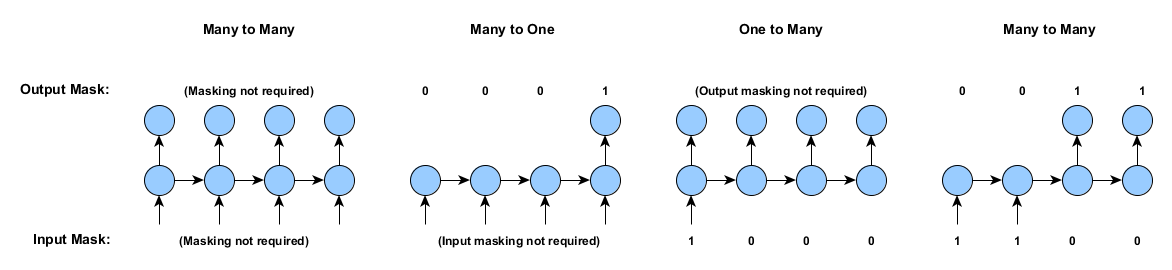
\includegraphics[width=\textwidth]{masking.png}
	\caption{Multiple masking methods \cite{dl4jRnn:online}}
	\label{fig:masking}
\end{figure} 


\subsection{Neural Network}
\label{sec:nn}

In this section we explain in more detail why Long-Short Term Memory (LSTM) \cite{lstmOrginin:article} networks handle the vanishing gradient problem, high dimensionality, and long-term dependencies. \\

First we briefly repeat the structure of a neural network in figure \ref{fig:nnStructure}. We see the input $x$, different layers with their neurons, $\sigma$ as the activation function, and $y$ as output. \\

\begin{figure}[!htb]
	\centering
	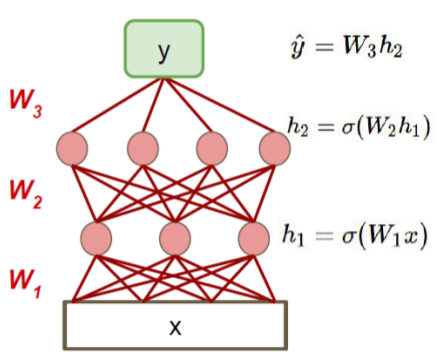
\includegraphics[width=0.6\textwidth]{nnStructure.png}
	\caption{General structure of a neural network \cite{IMECJaak}}
	\label{fig:nnStructure}
\end{figure} 

\subsubsection{Recurrent Neural Network}
\label{sec:rnn}

A standard neural network does not have any persistence. It will classify their input but when it gets a stream of inputs (ex. speech, video, \ldots), it will classify each word independently of each other and without any regards of the previous inputs. A recurrent neural network (RNN) addresses this problem by introducing networks with loops \cite{rnnOrigin:article}. This way, the output of a previous input has effect on the next input. In figure \ref{fig:rnnLoops}, we transform those loops into multiple copies of the same network which makes it easier to reason about. \\

\begin{figure}[!htb]
	\centering
	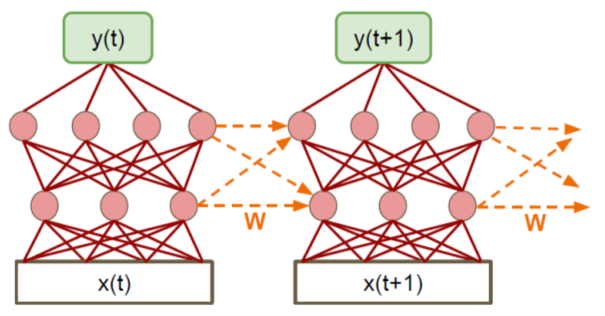
\includegraphics[width=0.7\textwidth]{rnnLoops.png}
	\caption{Unrolled recurrent neural network \cite{IMECJaak}}
	\label{fig:rnnLoops}
\end{figure} 

The problem with RNNs is mainly that they have trouble learning long-term dependencies which is often essential in time series \cite{longDepRNN:article}.


\subsubsection{Long Short Term Memory}
\label{sec:lstm}

A LSMT network is a specific RNN which is capable of learning long-term dependencies \cite{lstmDep:thesis}. We explain the difference with a standard RNN and why a LSTM can learn these long-term dependencies. \\

A recurrent network is, as we said, a chain of connected neural networks. Those networks can have a simple structure like a single $tanh$ layer, see figure \ref{fig:rnnTanh}. Representing a complete RNN as one layer which has neurons with activation function $tanh$, makes it easy to reason about. \\

\begin{figure}[!htb]
	\centering
	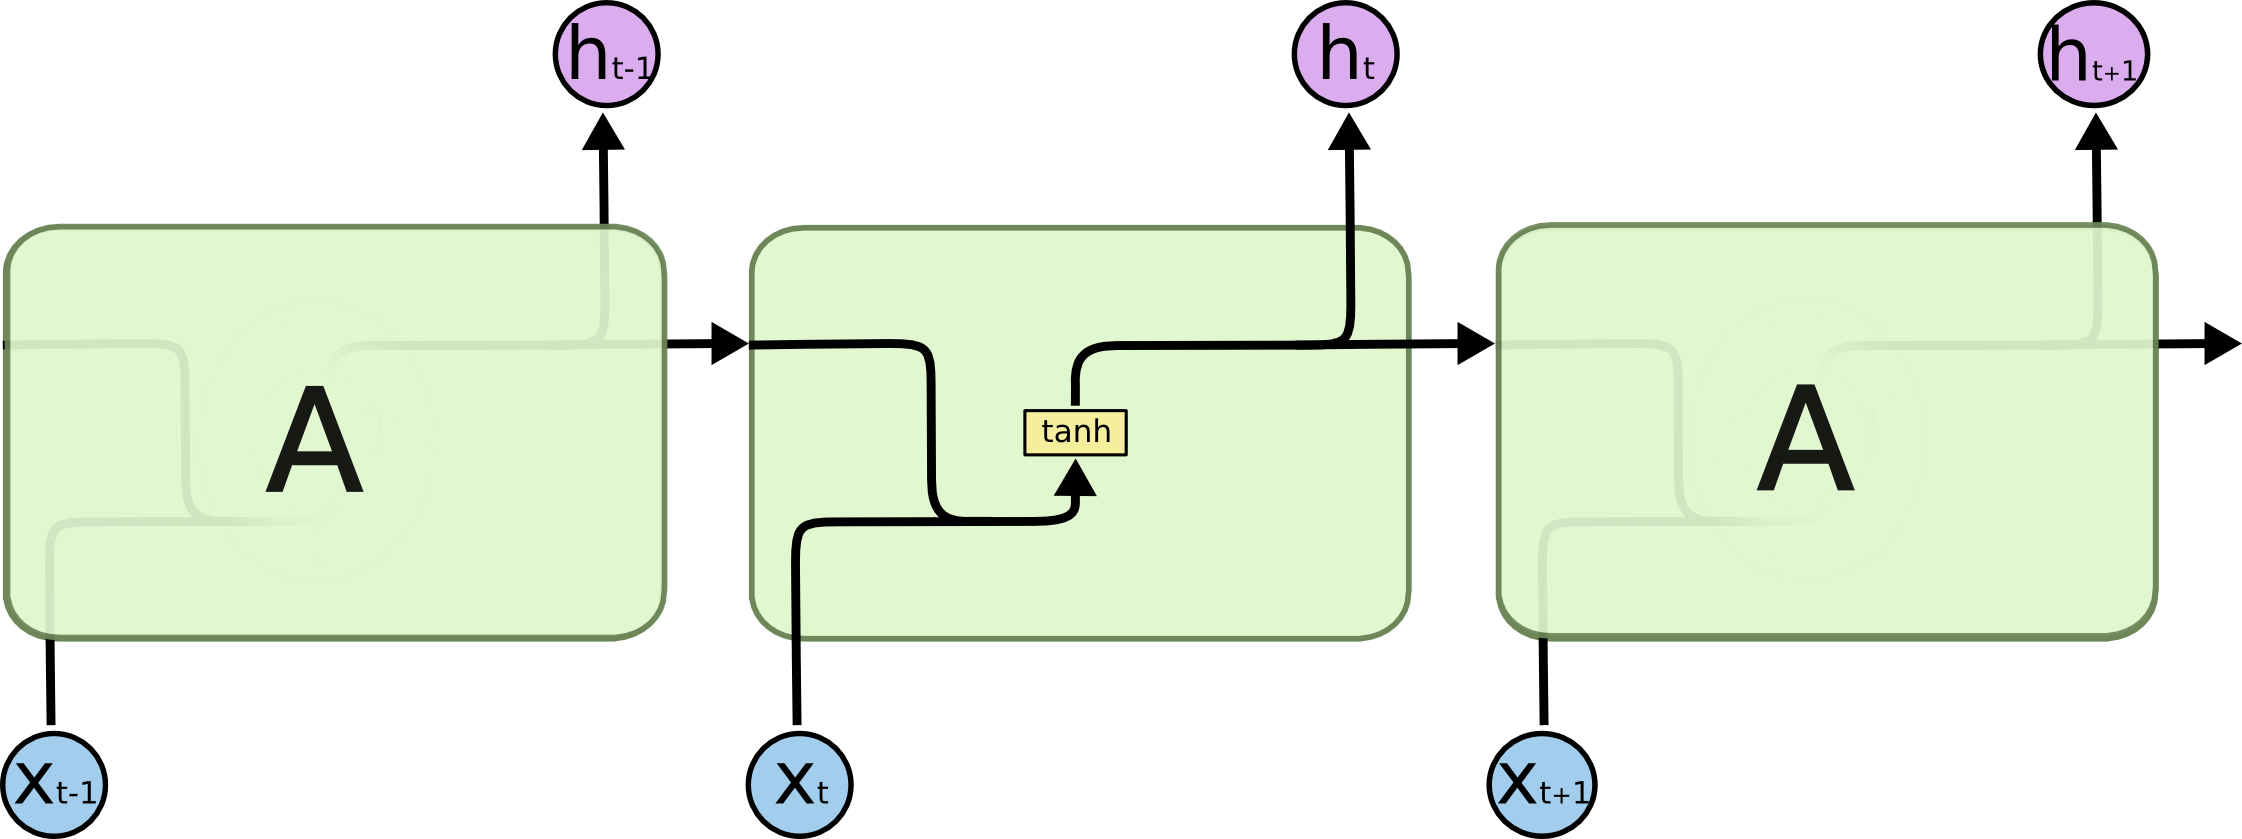
\includegraphics[width=0.7\textwidth]{rnnTanh.png}
	\caption{Unrolled recurrent neural network with a single tanh layer \cite{lstmGood:online}}
	\label{fig:rnnTanh}
\end{figure} 

It is important to see the difference with a LSTM. In this case the network does not have a single neural network layer, but has $4$ layers which each fulfill a specific goal, see figure \ref{fig:LSTMChain}.\\

\begin{figure}[!htb]
	\centering
	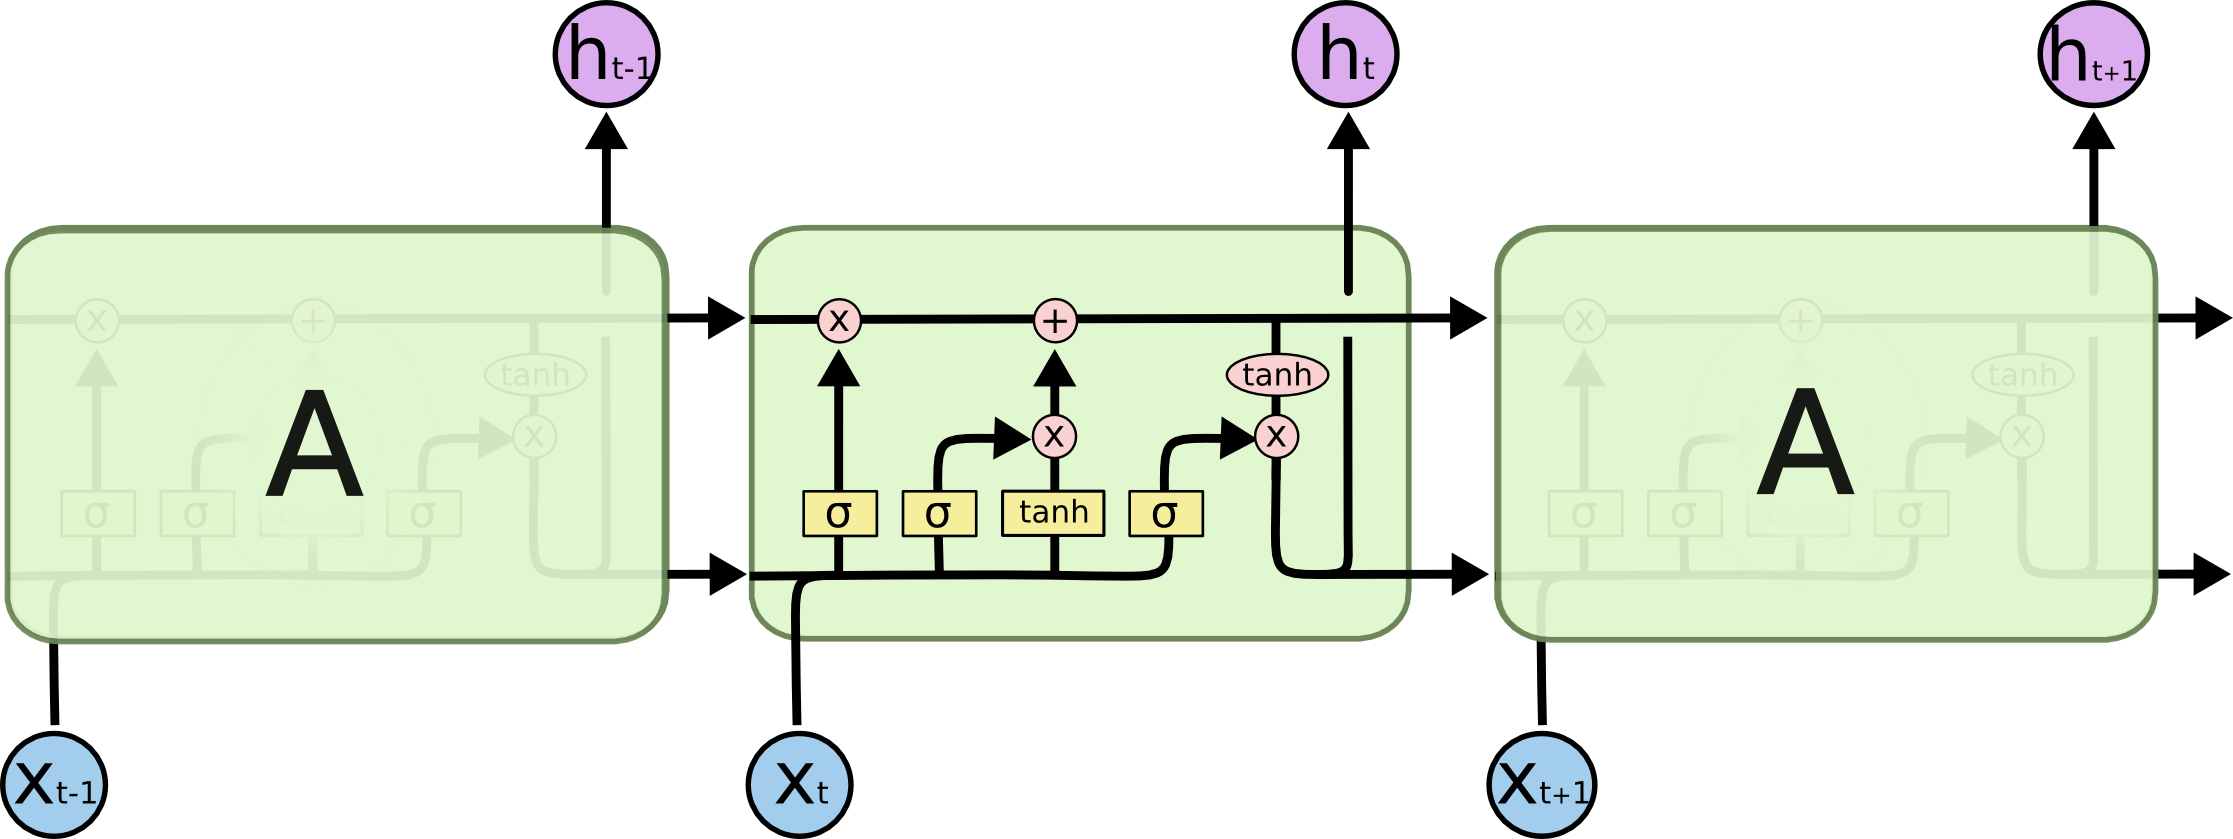
\includegraphics[width=0.7\textwidth]{LSTMChain.png}
	\caption{Unrolled LSTM network where each network has 4 layers \cite{lstmGood:online}}
	\label{fig:LSTMChain}
\end{figure} 

The main idea behind a LSTM is that each repeated network has its own \textit{cell state}. It functions as a memory which can be updated with each new input. In figure \ref{fig:LSTMConveyor}, you can see the \textit{cell state} $C$ through time. It can be compared with a conveyor belt which interacts with the input at certain gates. This way the state is updated throughout several inputs and this way a LSTM can keep track of long-term dependencies. \\

\begin{figure}[!htb]
	\centering
	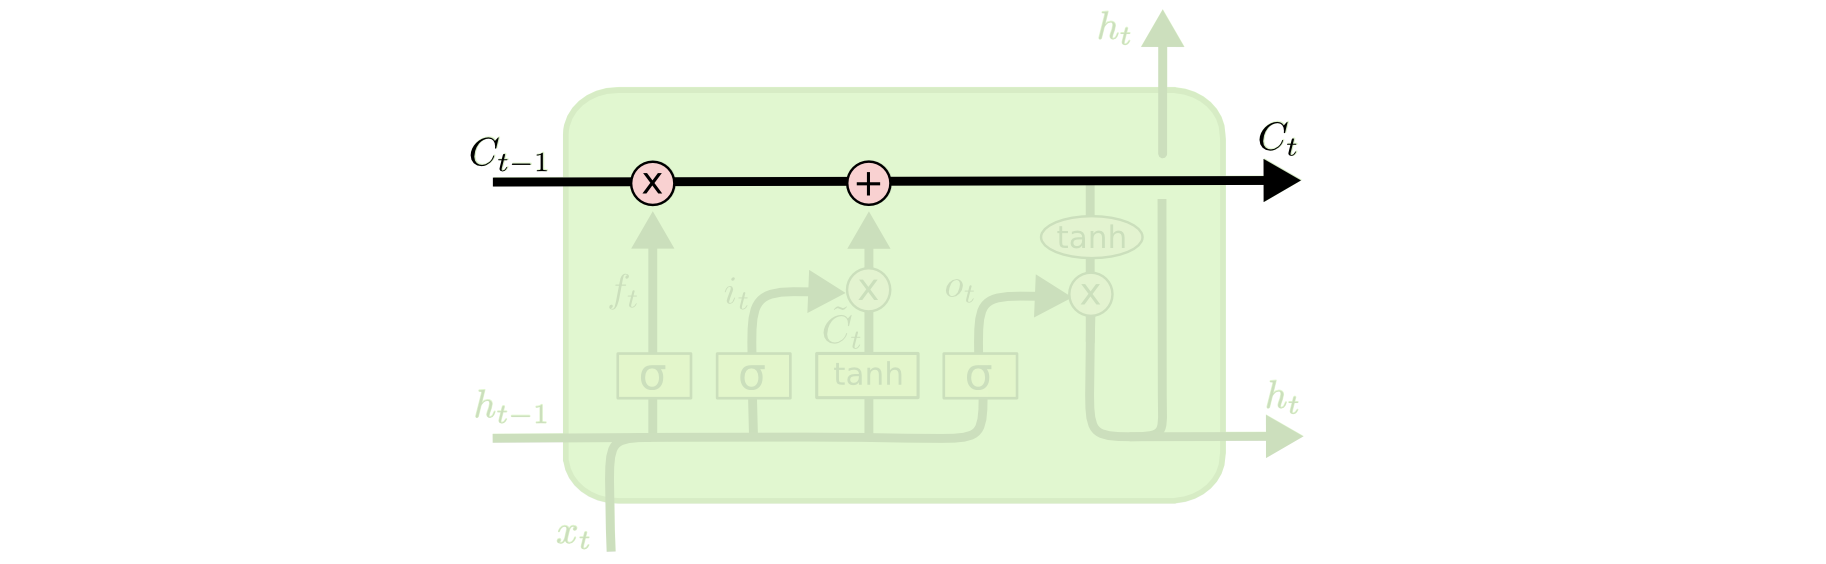
\includegraphics[width=0.7\textwidth]{LSTMConveyor.png}
	\caption{Representation of the cell state for a LSTM network \cite{lstmGood:online}}
	\label{fig:LSTMConveyor}
\end{figure} 

In the following figures, we show the different gates and their functions in changing the \textit{cell state} depending on the input and the output of the previous network. Next to each figure, formulas show how the \textit{cell state} is updated. There should be no surprises as they are not much different than the standard formulas of neural networks. \\

We start with the forget gate layer of a LSTM. Based on $x_t$ and $h_{t-1}$, it outputs a number between $0$ and $1$ for each number in the \textit{cell state} $C_{t-1}$. This is shown in figure \ref{fig:LSTM1}. When the output is $0$, the number in the \textit{cell state} is completely erased. With the output $1$, the number does not change. \\

\begin{figure}[!htb]
	\centering
	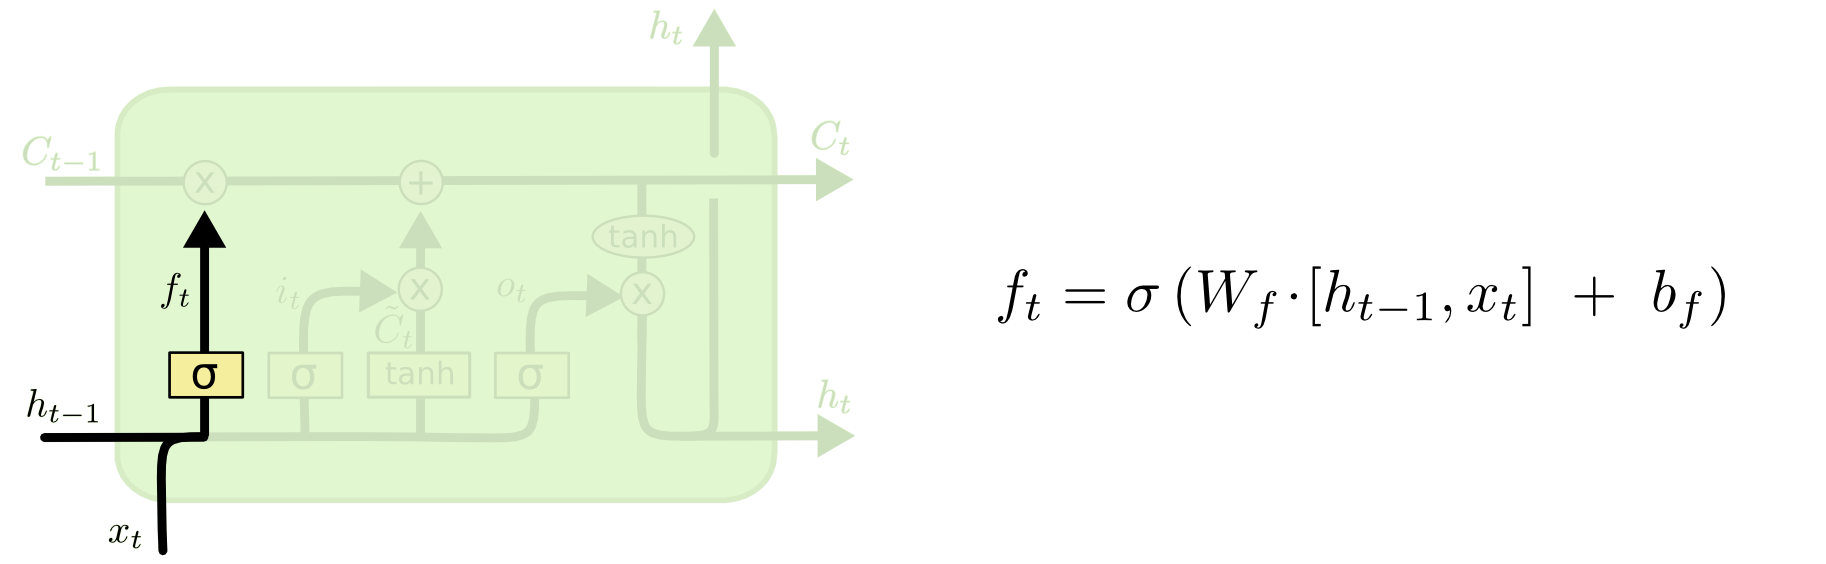
\includegraphics[width=0.7\textwidth]{LSTM1.png}
	\caption{Forget layer of a LSTM network \cite{lstmGood:online}}
	\label{fig:LSTM1}
\end{figure} 

Next we look to the input gate layer. This gate decides which values will be updated in the \textit{cell state} and outputs those in $i_t$. It is then combined with the vector $\widetilde{C}_t$, which contains the new candidate values based on the input $x_t$ and $h_{t-1}$. This is shown in figure \ref{fig:LSTM2}. \\

\begin{figure}[!htb]
	\centering
	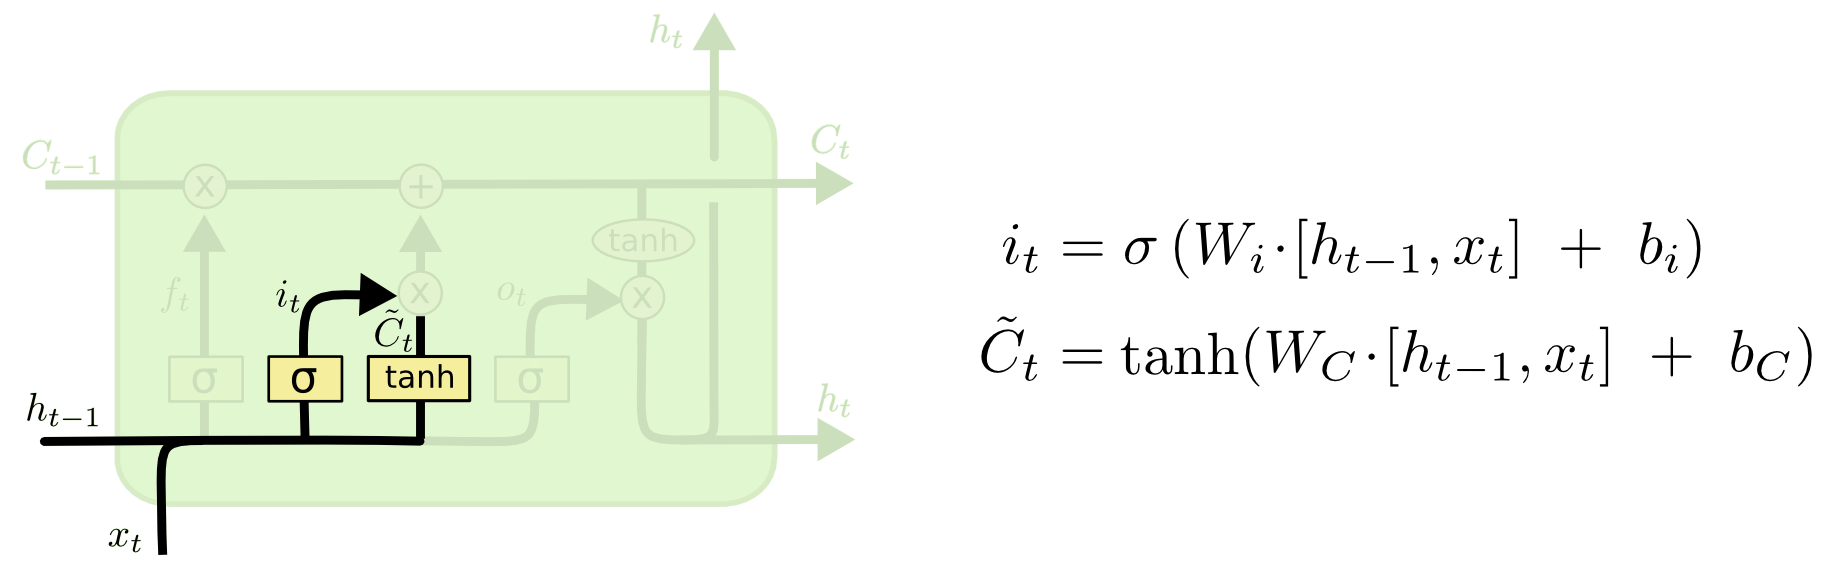
\includegraphics[width=0.7\textwidth]{LSTM2.png}
	\caption{Input layer of a LSTM network \cite{lstmGood:online}}
	\label{fig:LSTM2}
\end{figure} 

We can now combine the previous results and adjust the \textit{cell state}. We multiply the old state with $f_t$ so we forget the unneeded elements. Then we add $i_t*\widetilde{C}_t$ which are the new candidate values multiplied by the amount on how much we want to update each state value. See figure \ref{fig:LSTM3}. \\

\begin{figure}[!htb]
	\centering
	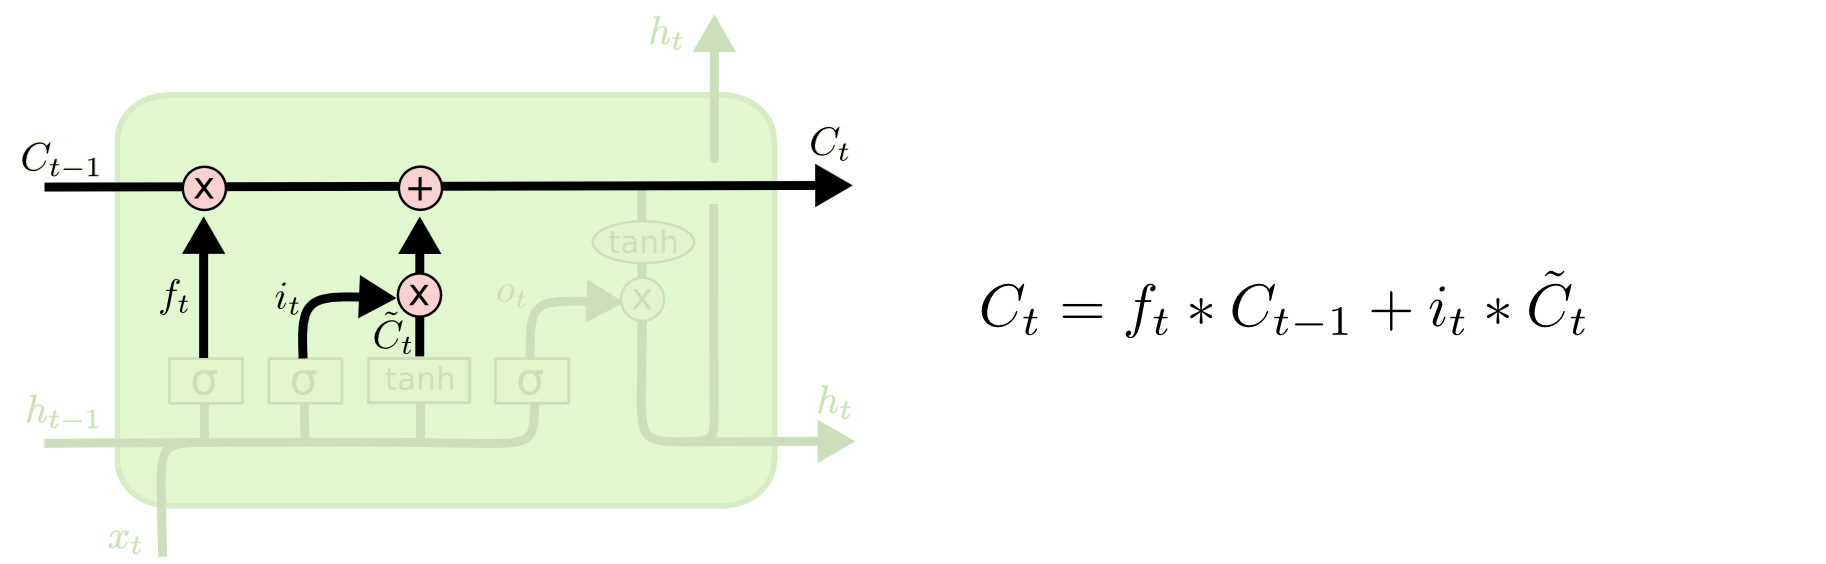
\includegraphics[width=0.7\textwidth]{LSTM3.png}
	\caption{Update process of the cell state of a LSTM network \cite{lstmGood:online}}
	\label{fig:LSTM3}
\end{figure} 

Finally, we need to output $h_t$ to the next network. This is based on the input and the \textit{cell state} $C_t$. See figure \ref{fig:LSTM4}. \\

\begin{figure}[!htb]
	\centering
	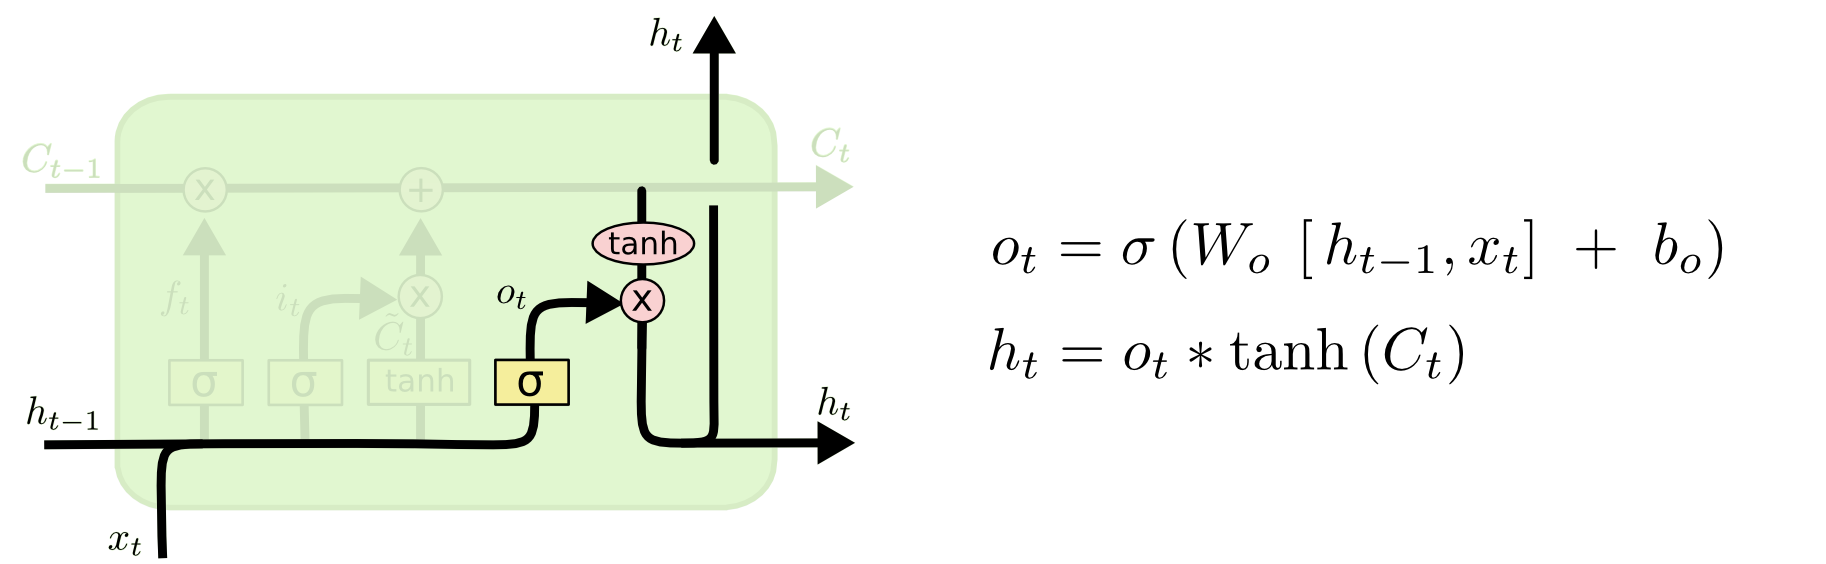
\includegraphics[width=0.7\textwidth]{LSTM4.png}
	\caption{Decide the output of a LSTM network \cite{lstmGood:online}}
	\label{fig:LSTM4}
\end{figure} 


\subsubsection{LSTM Variants}

In "LSTM: A Search Space Odyssey" \cite{lstmSpace:article}, different variants of LSTM networks are tested. It was concluded that the forget gate and the activation function are the most important parts. Other variants do not have a large influence and mainly add extra complexity.


\section{Conclusion}

In this chapter we talked about improvements such as a better categorization approach and the use of data distribution. \\
We mainly focused on LSTM neural networks and explained why they should be suitable to predict or classify disease trajectories. They are able to handle the Curse of Dimensionality, long time dependencies, and take the temporal aspect of medical data into account. Our Word2Vec approaches can be used in combination with this kind of neural network. The prediction/classification accuracy of the LSMT neural network makes it possible to validate the working of our approaches by testing if the accuracy increases with the use of generalized Word2Vec approaches. 


%%% Local Variables: 
%%% mode: latex
%%% TeX-master: "thesis"
%%% End: 


% If you have appendices:
%\appendixpage*          % if wanted
%\appendix
%\chapter{The First Appendix}
\label{app:A}
Appendices hold useful data which is not essential to understand the work
done in the master thesis. An example is a (program) source.
An appendix can also have sections as well as figures and references\cite{h2g2}.

\section{More Lorem}
\lipsum[50]

\subsection{Lorem 15--17}
\lipsum[15-17]

\subsection{Lorem 18--19}
\lipsum[18-19]

\section{Lorem 51}
\lipsum[51]

%%% Local Variables: 
%%% mode: latex
%%% TeX-master: "thesis"
%%% End: 

% ... and so on until
%\chapter{De laatste bijlage}
\label{app:n}
In de bijlagen vindt men de data terug die nuttig kunnen zijn voor de
lezer, maar die niet essentieel zijn om het betoog in de normale tekst te
kunnen volgen. Voorbeelden hiervan zijn bronbestanden,
configuratie-informatie, langdradige wiskundige afleidingen, enz.

\section{Lorem 20-24}
\lipsum[20-24]

\section{Lorem 25-27}
\lipsum[25-27]

%%% Local Variables: 
%%% mode: latex
%%% TeX-master: "masterproef"
%%% End: 


%test \cite{WHO_ICD}

\backmatter
% The bibliography comes after the appendices.
% You can replace the standard "abbrv" bibliography style by another one.
\nocite{*}
\bibliographystyle{abbrv}
\bibliography{references}

\end{document}

%%% Local Variables: 
%%% mode: latex
%%% TeX-master: t
%%% End: 
